\documentclass[11pt,conference,a4paper]{IEEEtran}
\usepackage{xeCJK}
\setCJKmainfont{SimSun}
\setCJKsansfont{SimHei}
\setCJKmonofont{SimSun}
\usepackage{fontspec}
\setmainfont{Times New Roman}
\usepackage{graphicx}
\graphicspath{{./}{../results/training/}}
\usepackage{booktabs}
\usepackage{tabularx}
\usepackage{array}
\usepackage{float}
\usepackage{caption}
\captionsetup{font=footnotesize,labelfont=bf,labelsep=period,justification=centering}
\usepackage[table]{xcolor}
\definecolor{Ink}{HTML}{1F2937}
\definecolor{Accent}{HTML}{0F766E}
\definecolor{AccentLight}{HTML}{F0F7F6}
\definecolor{Rule}{HTML}{CBD5E1}
\definecolor{Muted}{HTML}{64748B}
\usepackage{url}
\usepackage{hyperref}
\hypersetup{colorlinks=true,linkcolor=Accent,urlcolor=Accent}
\usepackage{microtype}
\usepackage{placeins}
\usepackage{flushend}
\usepackage{enumitem}
\setlist[itemize]{leftmargin=1.2em,itemsep=0.1em,topsep=0.1em}
\setlist[enumerate]{leftmargin=1.8em,itemsep=0.15em,topsep=0.1em}
\usepackage{tikz}
\usetikzlibrary{arrows.meta,positioning}
\newcommand{\code}[1]{\texttt{\footnotesize #1}}
\newcommand{\markterm}[1]{\textcolor{Accent}{\textbf{#1}}}
\newcommand{\tightcaption}[1]{\caption{#1}\vspace{-0.4em}}
\renewcommand{\arraystretch}{1.12}
\renewcommand{\figurename}{图}
\renewcommand{\tablename}{表}
\begin{document}

\title{实验一：基于 YOLOv8 与 Jetson 的四类桌面物体检测系统}
\author{\IEEEauthorblockN{机器人学集成小组项目}
\IEEEauthorblockA{中国海洋大学计算机科学与技术学院\\
个人 GitHub：\url{https://github.com/9161942-boop/robotics-experiment-1}}}
\maketitle

\begin{abstract}
本文报告一个面向桌面物体的端到端目标检测系统。实验从视频抽帧和 ISAT 人工标注开始，经 YOLO detection 格式转换，在四类自定义数据上训练 YOLOv8n，并将最佳权重部署到 Jetson Orin。系统同时保留 mouse、laptop、cup、phone 四类输出，通过 ROS2 发布 \code{/detections}。在完全独立的 80 张实物照片上，系统通过 72 张，图片级准确率为 90\%；Jetson 演示视频显示约 15 FPS。报告同时给出数据、训练、独立测试、部署、错误案例和 GitHub 分阶段提交证据。
\end{abstract}

\begin{IEEEkeywords}
目标检测，YOLOv8，Jetson，ROS2，独立实物测试，实验报告
\end{IEEEkeywords}

\section{实验目标与系统概览}
本实验的目标是建立一套可运行、可复现、可验收的桌面物体检测链路。系统输入为摄像头图像，核心模型为四类 YOLOv8n，输出包含类别、边界框和置信度，并在 Jetson 上实时显示。完整链路为：\markterm{摄像头采集} $\rightarrow$ \markterm{YOLOv8 检测} $\rightarrow$ \markterm{Jetson 实时显示} $\rightarrow$ \markterm{ROS2 发布}。

\begin{quote}\small
\textbf{验收结果：}独立实物照片测试 72/80（90\%），高于 80\% 门槛；Jetson 视频画面显示约 15 FPS，高于 5 FPS 门槛；数据集、模型、程序、视频、运行说明和错误案例均已归档。
\end{quote}

\FloatBarrier
\section{完整实验流程}
实验遵循“采集—标注—转换—训练—验证—部署—验收—归档”的顺序。每一步均产生可追溯文件，最终通过 GitHub 分阶段 commit 固化。

\begin{figure}[H]
\centering
\resizebox{\columnwidth}{!}{%
\begin{tikzpicture}[
  flow/.style={draw=Ink,fill=AccentLight,rounded corners=1mm,minimum width=2.75cm,minimum height=0.62cm,align=center,font=\small\bfseries,text=Ink},
  arrow/.style={-{Stealth[length=2mm]},semithick,color=Accent}
]
\node[flow] (a) {1. 采集与筛选};
\node[flow,right=0.38cm of a] (b) {2. ISAT 标注};
\node[flow,right=0.38cm of b] (c) {3. YOLO 转换};
\node[flow,right=0.38cm of c] (d) {4. YOLOv8 训练};
\node[flow,below=0.45cm of d] (e) {5. 验证与诊断};
\node[flow,left=0.38cm of e] (f) {6. 独立实物测试};
\node[flow,left=0.38cm of f] (g) {7. Jetson 部署};
\node[flow,left=0.38cm of g] (h) {8. ROS2 发布};
\draw[arrow] (a)--(b)--(c)--(d);
\draw[arrow] (d)--(e)--(f)--(g)--(h);
\end{tikzpicture}}
\tightcaption{从原始视频到可验收系统的完整实验流程}
\end{figure}

\begin{enumerate}
\item 从桌面物体视频中抽帧，筛选清晰且具有不同角度、距离和背景的样本，形成四类原始图片。
\item 使用 ISAT 绘制边界框并检查类别一致性，保存原始图片和 JSON 标注。
\item 将 ISAT 标注转换为 YOLO detection 格式，按 train/val/test 划分并检查标签数量。
\item 以 COCO 预训练 YOLOv8n 为初始化训练 100 个 epoch，记录参数、曲线和最佳权重。
\item 在验证集和 test 诊断集上计算 Precision、Recall、mAP，并保存漏检与误检案例。
\item 使用完全未参与训练的 80 张独立实物照片进行图片级筛查，统计各类别和总体通过率。
\item 将四类权重部署到 Jetson Orin，运行摄像头程序，检查检测框、类别、置信度和 FPS。
\item 通过 ROS2 节点把图像检测结果封装为 Detection2DArray 并发布到 \code{/detections}，最后整理报告和 GitHub 记录。
\end{enumerate}

\FloatBarrier
\section{硬件、软件与数据集}
\begin{table}[H]
\centering
\scriptsize
\caption{实验环境与数据配置}
\begin{tabularx}{\columnwidth}{>{\bfseries}p{0.23\columnwidth} X}
\toprule
训练平台 & Windows 11 + RTX 4060 Laptop GPU\\
部署平台 & Jetson Orin，Ubuntu 20.04\\
框架与版本 & YOLOv8n，Ultralytics 8.4.22\\
ROS2 & Humble，消息为 \code{Detection2DArray}\\
输入图像 & 640$\times$480 USB 摄像头\\
类别与规模 & mouse / laptop / cup / phone；图像总数 595（421/87/87）\\
\bottomrule
\end{tabularx}
\end{table}

数据来自桌面物体视频抽帧，经 ISAT 标注并转换为 YOLO detection 格式。训练、验证和测试划分相互独立，测试集没有参与训练。图~\ref{fig:annotation} 给出四类样本及其人工边界框。

\begin{figure}[H]
\centering
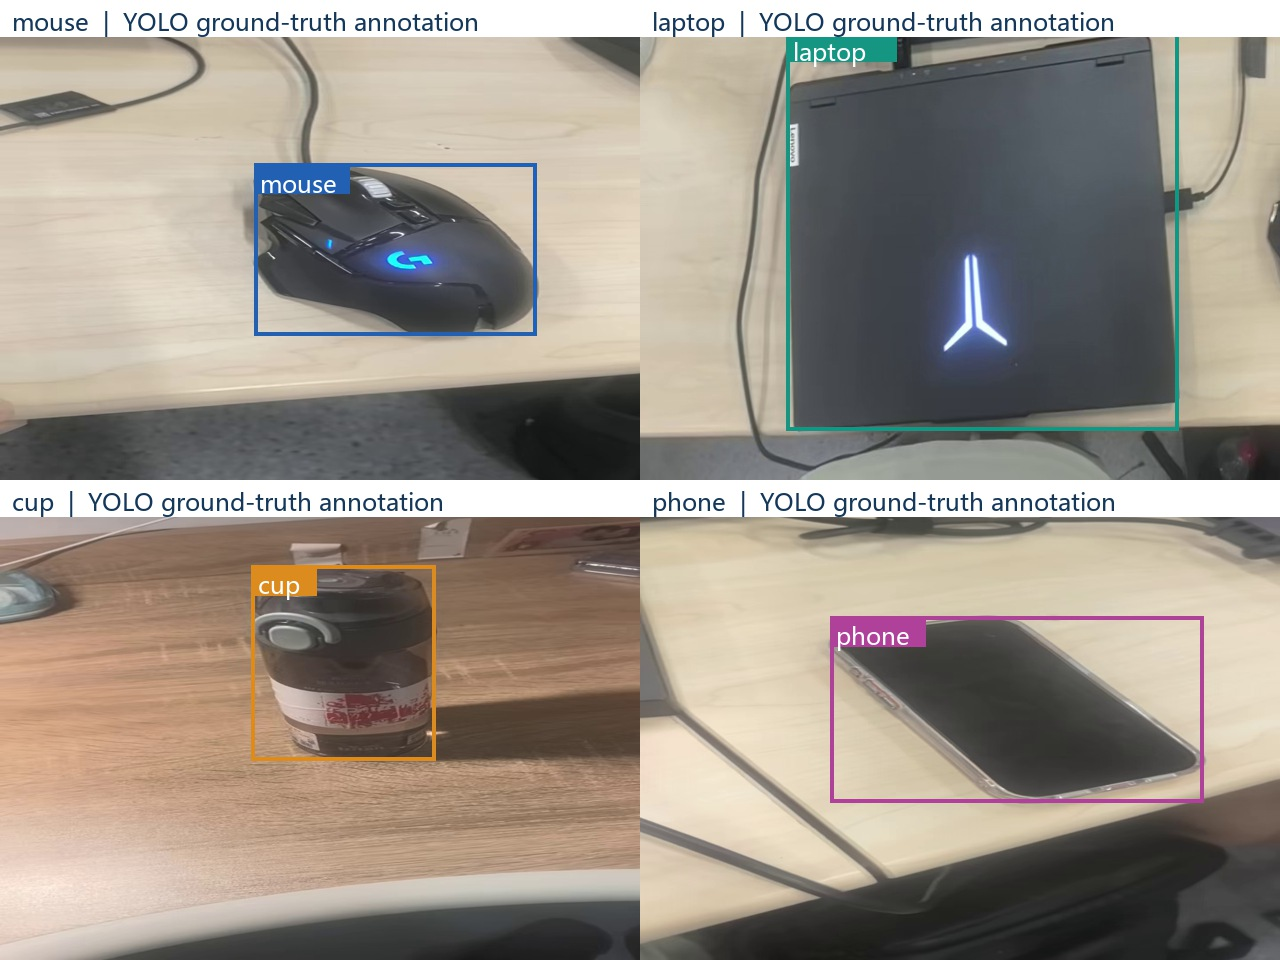
\includegraphics[width=0.98\columnwidth]{dataset_annotation_examples.jpg}
\tightcaption{数据集样本与人工标注框示例}
\label{fig:annotation}
\end{figure}

\FloatBarrier
\section{训练方法与模型质量}
以 COCO 预训练 YOLOv8n 为初始化，在四类数据集上训练 100 个 epoch，输入尺寸 640，batch size 16，推理置信度阈值 0.25；Jetson 演示使用 0.35。训练配置、曲线和最佳权重保存在仓库中，最终模型为四类输出的 \code{weights/best.pt}。

\begin{figure}[H]
\centering
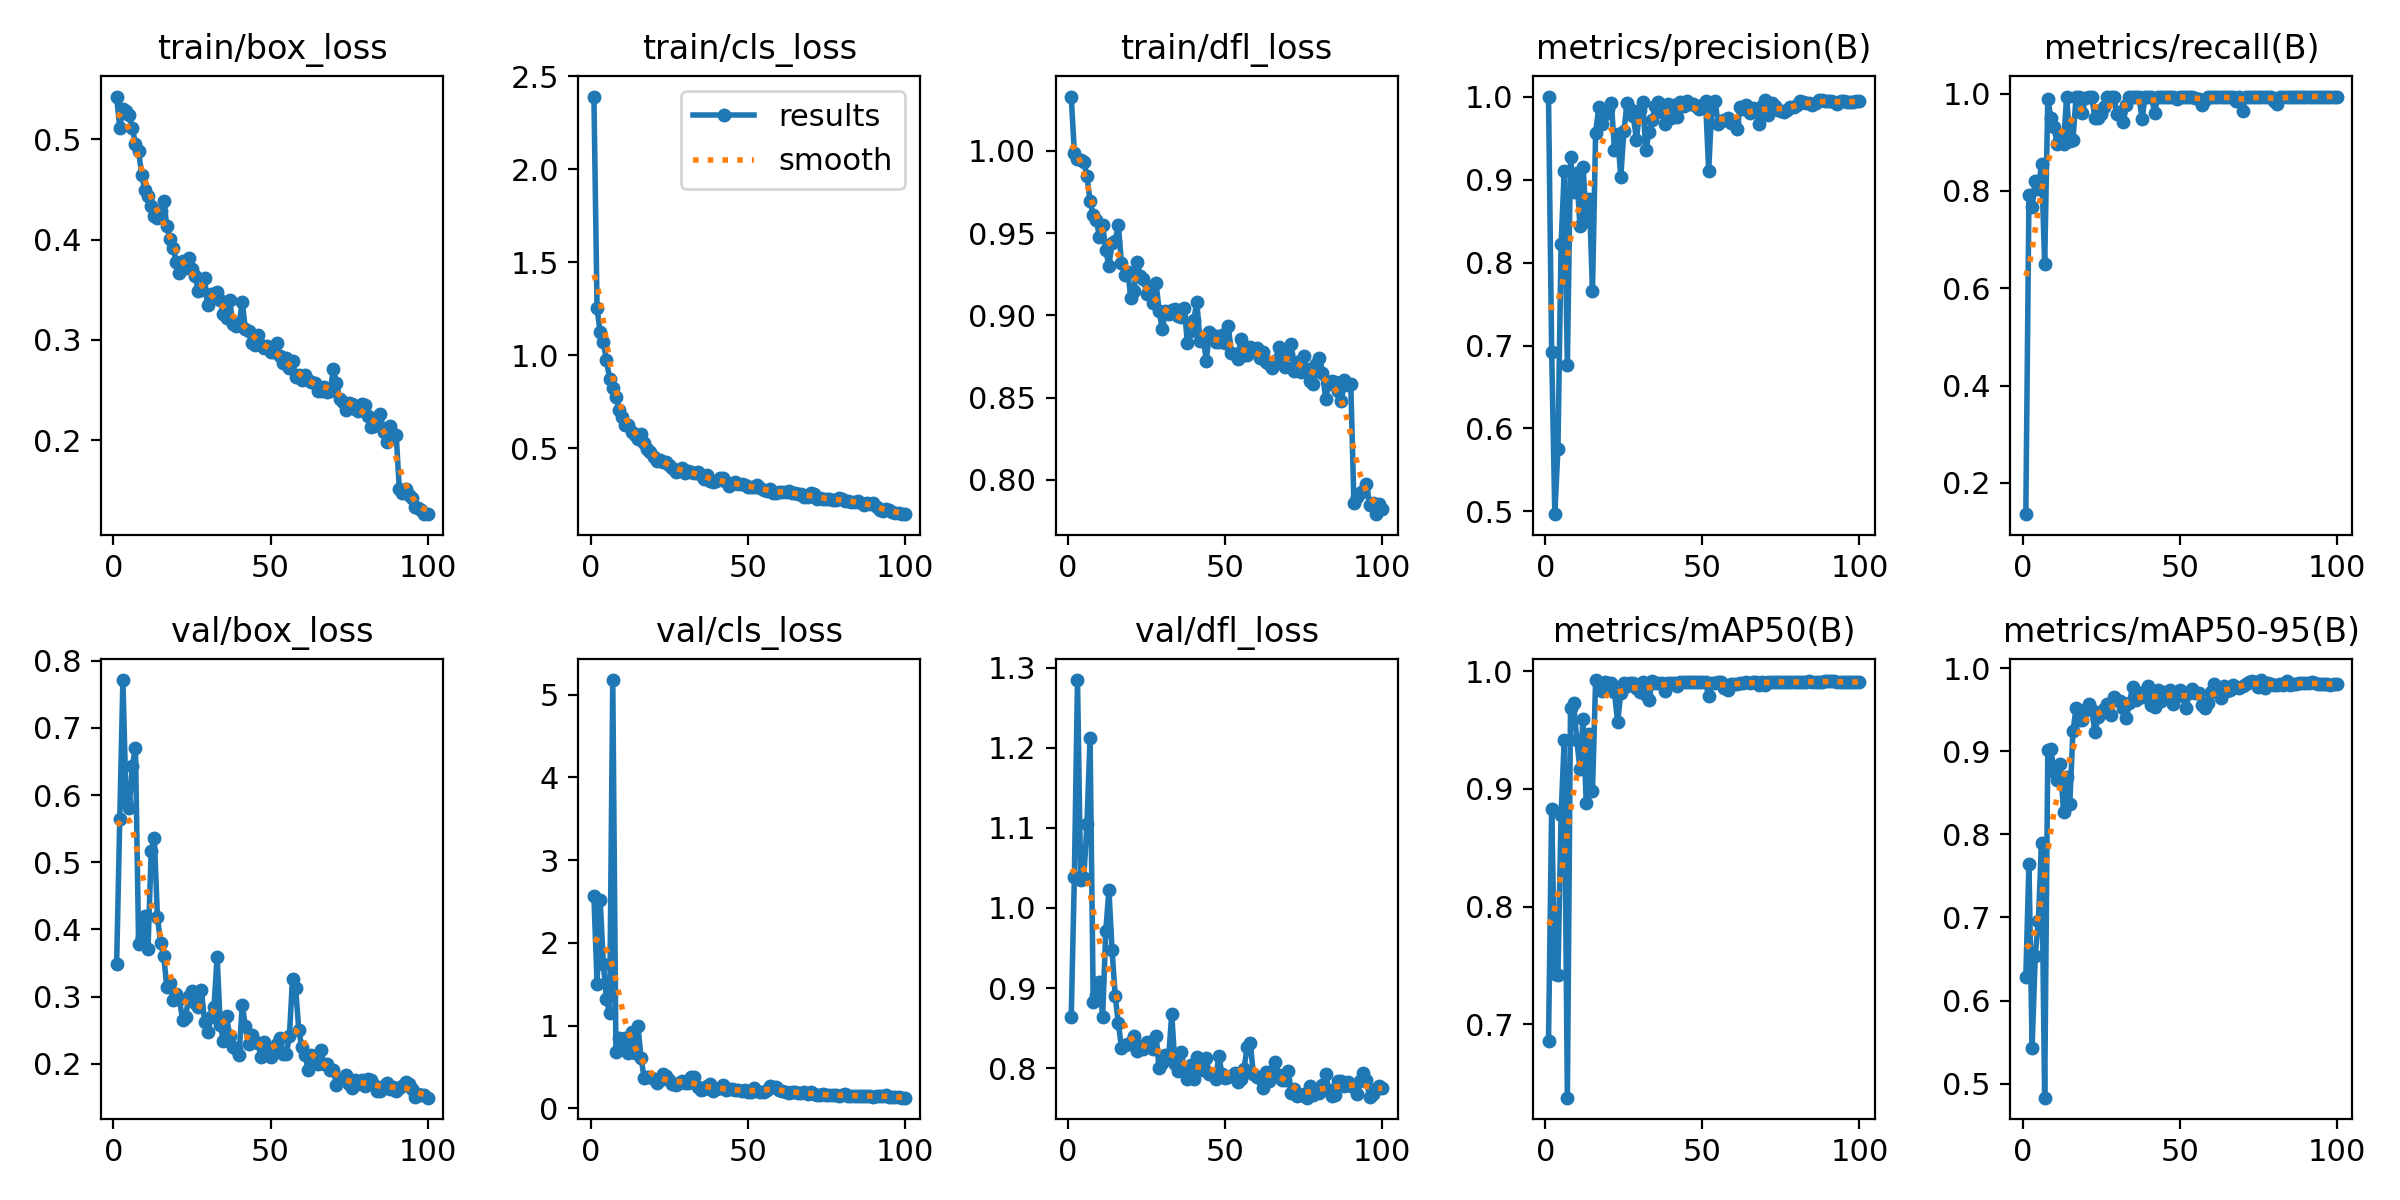
\includegraphics[width=0.98\columnwidth]{results.png}
\tightcaption{训练过程指标曲线（对应仓库 \code{results/training/results.png}）}
\end{figure}

\begin{table}[H]
\centering
\scriptsize
\setlength{\tabcolsep}{2.5pt}
\caption{验证集与诊断集结果}
\begin{tabular}{lcccc}
\toprule
数据/指标 & P & R & mAP@50 & mAP@50:95\\
\midrule
dataset/yolo 验证集 & 0.658 & 0.748 & 0.766 & 0.701\\
\bottomrule
\end{tabular}
\end{table}

\begin{figure}[H]
\centering
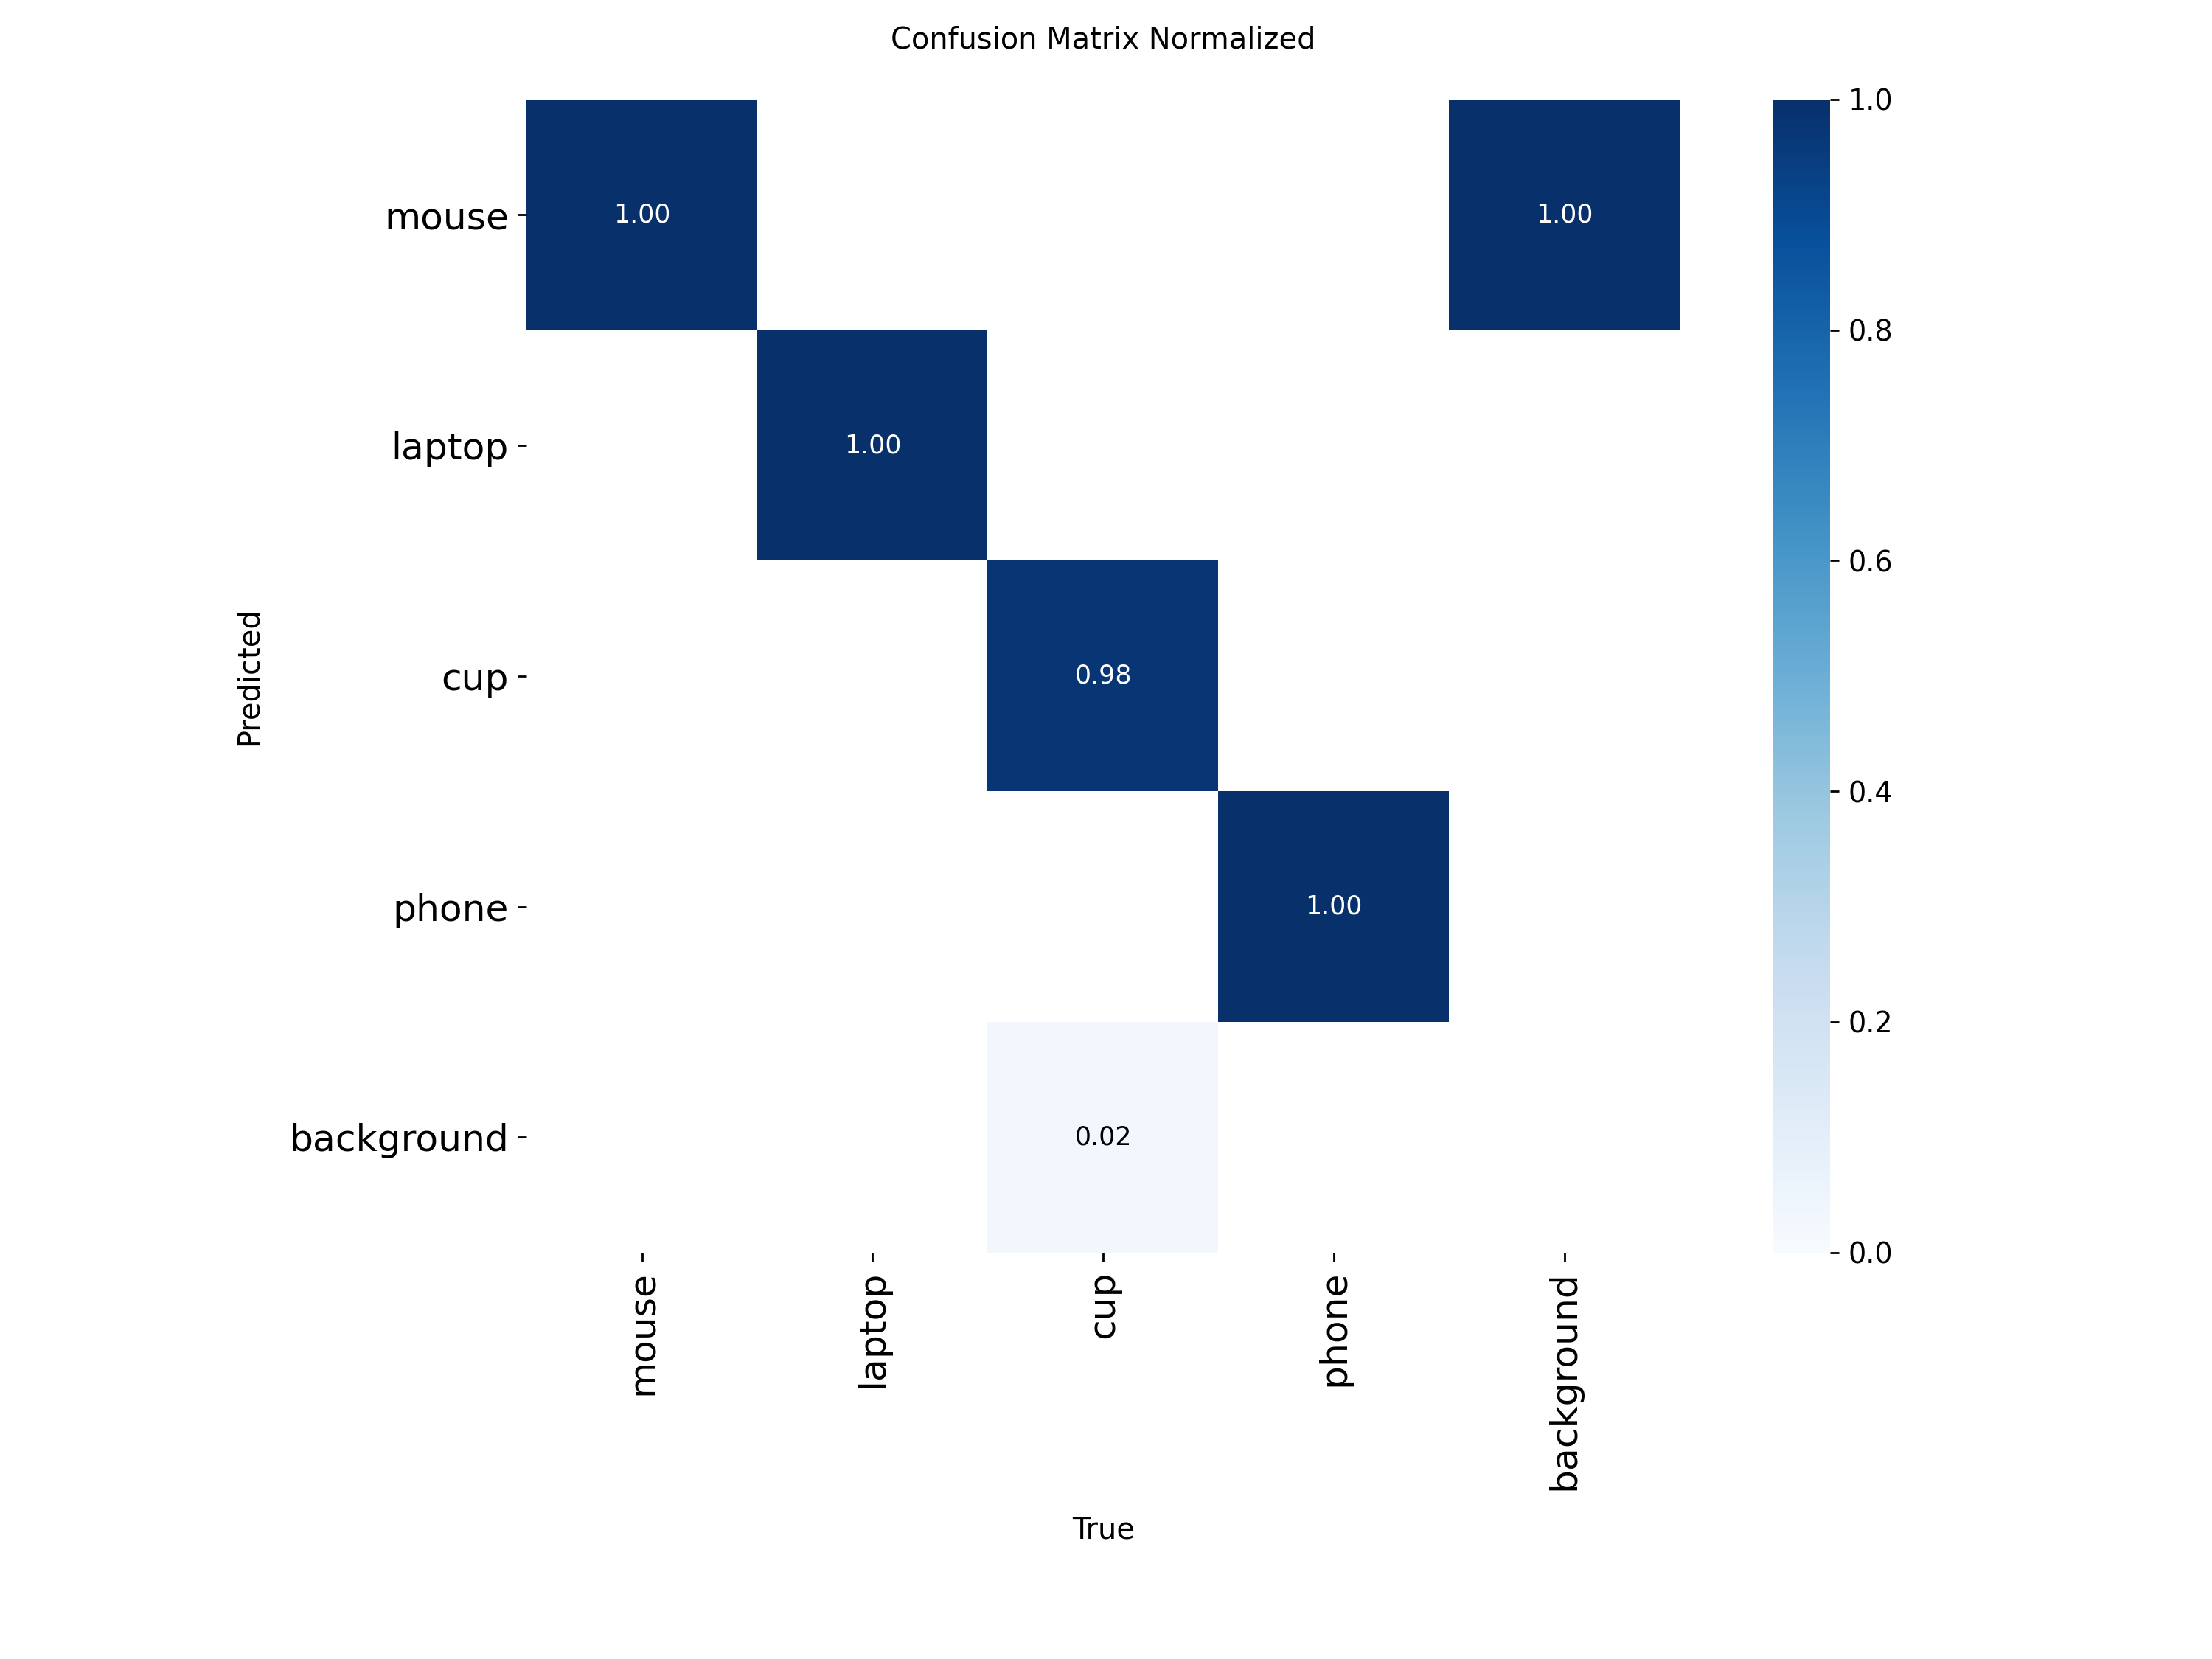
\includegraphics[width=0.72\columnwidth]{confusion_matrix_normalized.png}
\tightcaption{四类目标的归一化混淆矩阵}
\end{figure}

独立验收集共 80 张照片，每个类别 20 张，按“该照片中目标是否被正确识别”统计：cup 17/20、laptop 19/20、mouse 18/20、phone 18/20，总计 72/80（90\%）。未通过样本为 \code{04\_cup.jpg}、\code{12\_cup.jpg}、\code{13\_cup.jpg}、\code{21\_laptop.jpg}、\code{42\_mouse.jpg}、\code{46\_mouse.jpg}、\code{72\_phone.jpg}、\code{80\_phone.jpg}。

\begin{figure}[H]
\centering
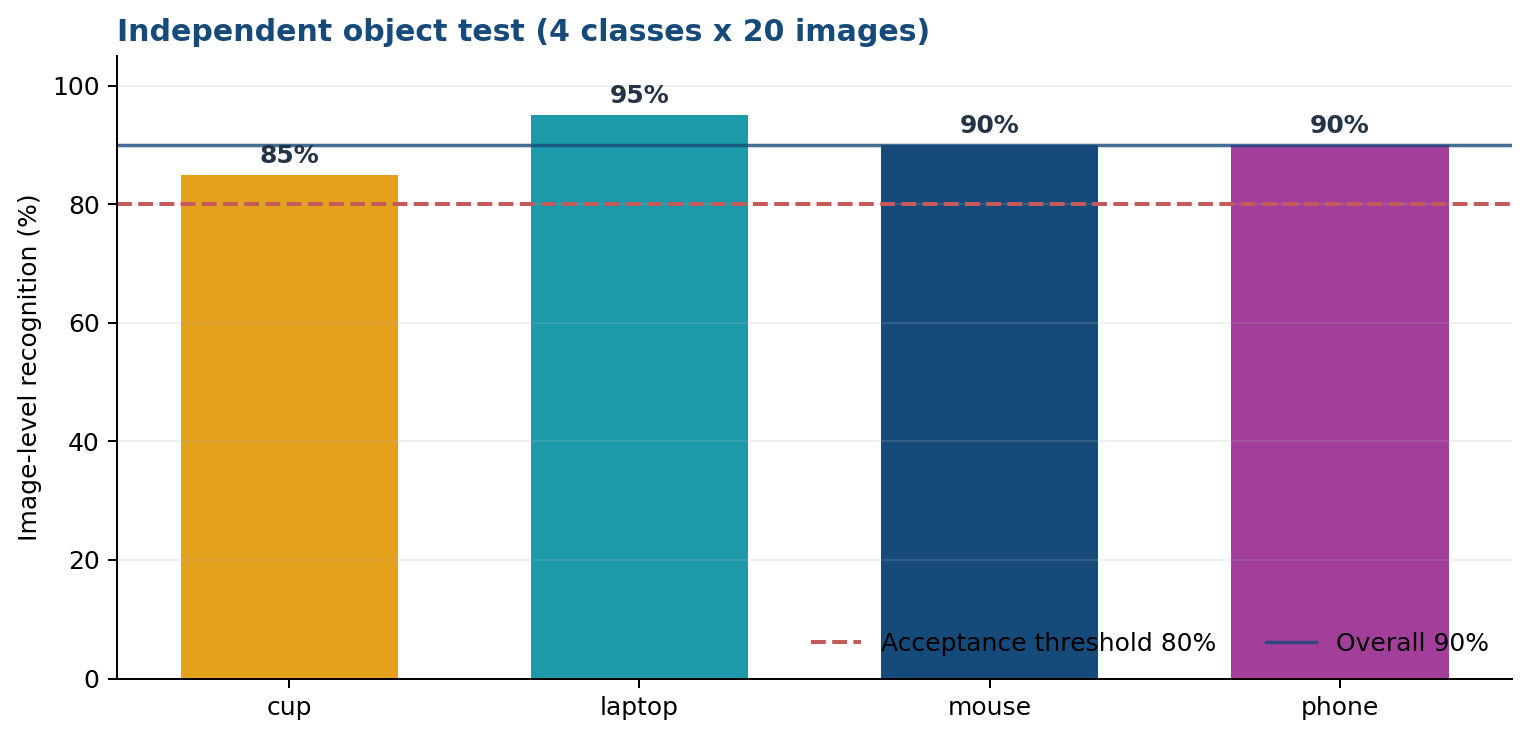
\includegraphics[width=0.98\columnwidth]{independent_accuracy.png}
\tightcaption{80 张独立实物照片的分类型通过率与 80\% 验收门槛}
\end{figure}

\FloatBarrier
\section{Jetson 部署与 ROS2 发布}
Jetson 演示视频分辨率为 640$\times$480，画面叠加检测框、类别、置信度和 FPS。原视频中的 FPS 显示约 15.0，满足不低于 5 FPS 的验收要求；抽帧中可同时看到 mouse、phone、laptop 和 cup 的检测框。

\begin{figure}[H]
\centering
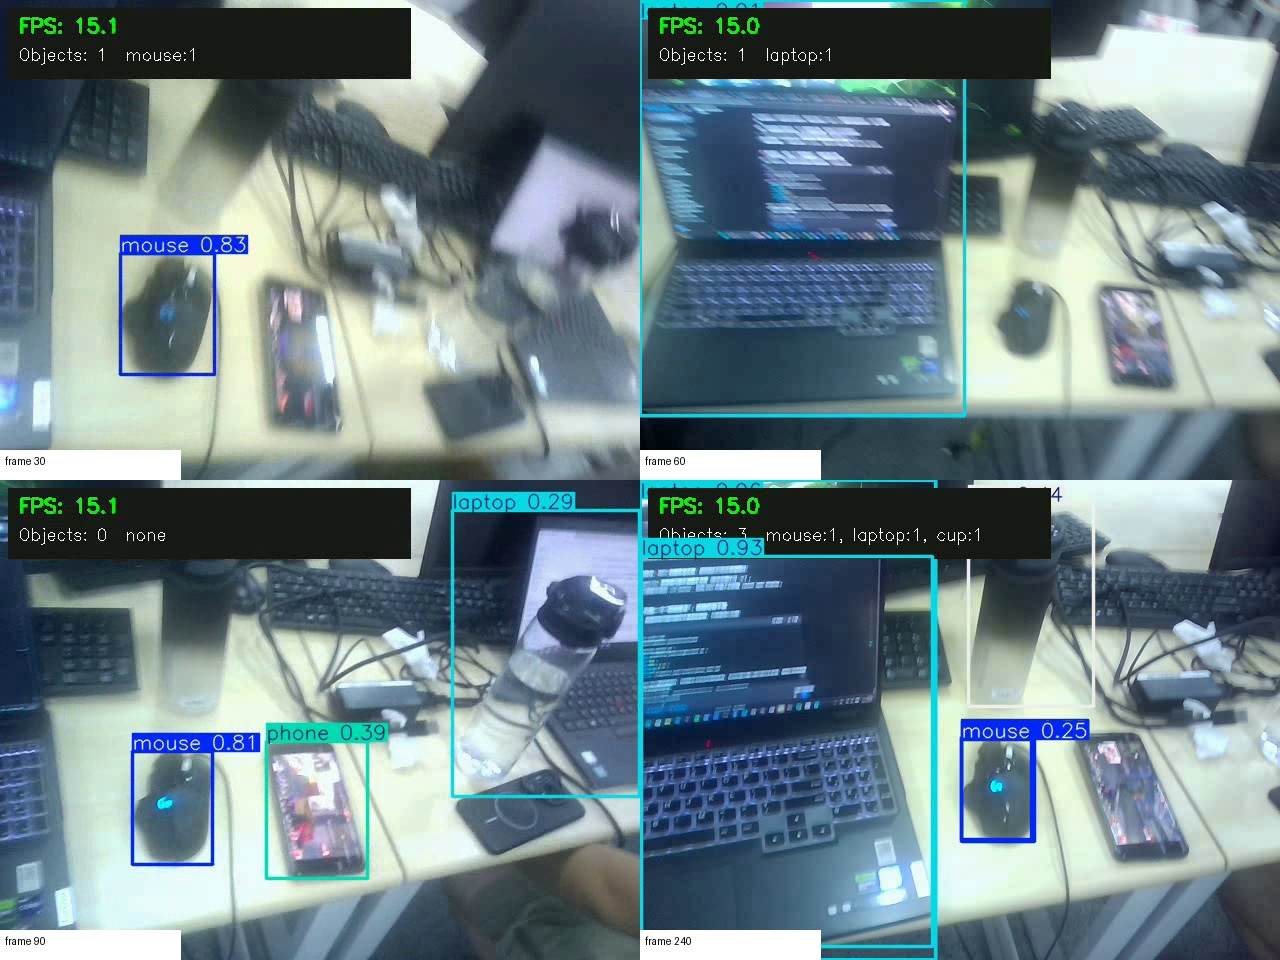
\includegraphics[width=0.98\columnwidth]{jetson_demo_montage.jpg}
\tightcaption{Jetson 演示视频抽帧（原视频：\code{results/videos/jetson\_demo.mp4}）}
\end{figure}

检测节点订阅 \code{/camera/image\_raw}，推理后发布 \code{/detections}（\code{vision\_msgs/Detection2DArray}）。程序、启动方式、参数和验证命令写入 \code{docs/ros2\_quickstart.md}，现场验证命令为：
\begin{quote}\small\code{ros2 topic echo /detections --once}\end{quote}

\FloatBarrier
\section{错误分析与可复现性}
错误案例已保存于 \code{results/independent\_test\_80/errors/} 和 \code{results/evaluation\_final/errors/}。失败主要与小目标、运动模糊、遮挡和低置信度有关。后续可补充困难样本、提高输入尺寸、增加数据增强，并使用 TensorRT 优化部署速度。

\FloatBarrier
\section{GitHub 提交记录与材料追踪}
按照课程要求，报告、数据、代码、模型和结果均上传至个人 GitHub，并保留分阶段 commit 记录，未采用一次性全量提交。仓库链接为：\url{https://github.com/9161942-boop/robotics-experiment-1}。

\begin{table}[H]
\centering
\scriptsize
\caption{代表性分阶段提交}
\begin{tabularx}{\columnwidth}{>{\bfseries}p{0.20\columnwidth} p{0.20\columnwidth} X}
\toprule
阶段 & Commit & 内容\\
\midrule
数据准备 & \code{5fcd148} & 鼠标样本与标注计划\\
数据准备 & \code{c2507b4} & cup/laptop/phone 数据补充\\
训练管线 & \code{3e007d8} & 四类 YOLO 训练流程\\
独立测试 & \code{a93ffb5} & 独立图片筛查记录\\
Jetson 部署 & \code{14a710c} & 实时检测演示视频\\
验收整理 & \code{d887607} & 验收材料与 PDF 报告\\
\bottomrule
\end{tabularx}
\end{table}

\begin{figure}[H]
\centering
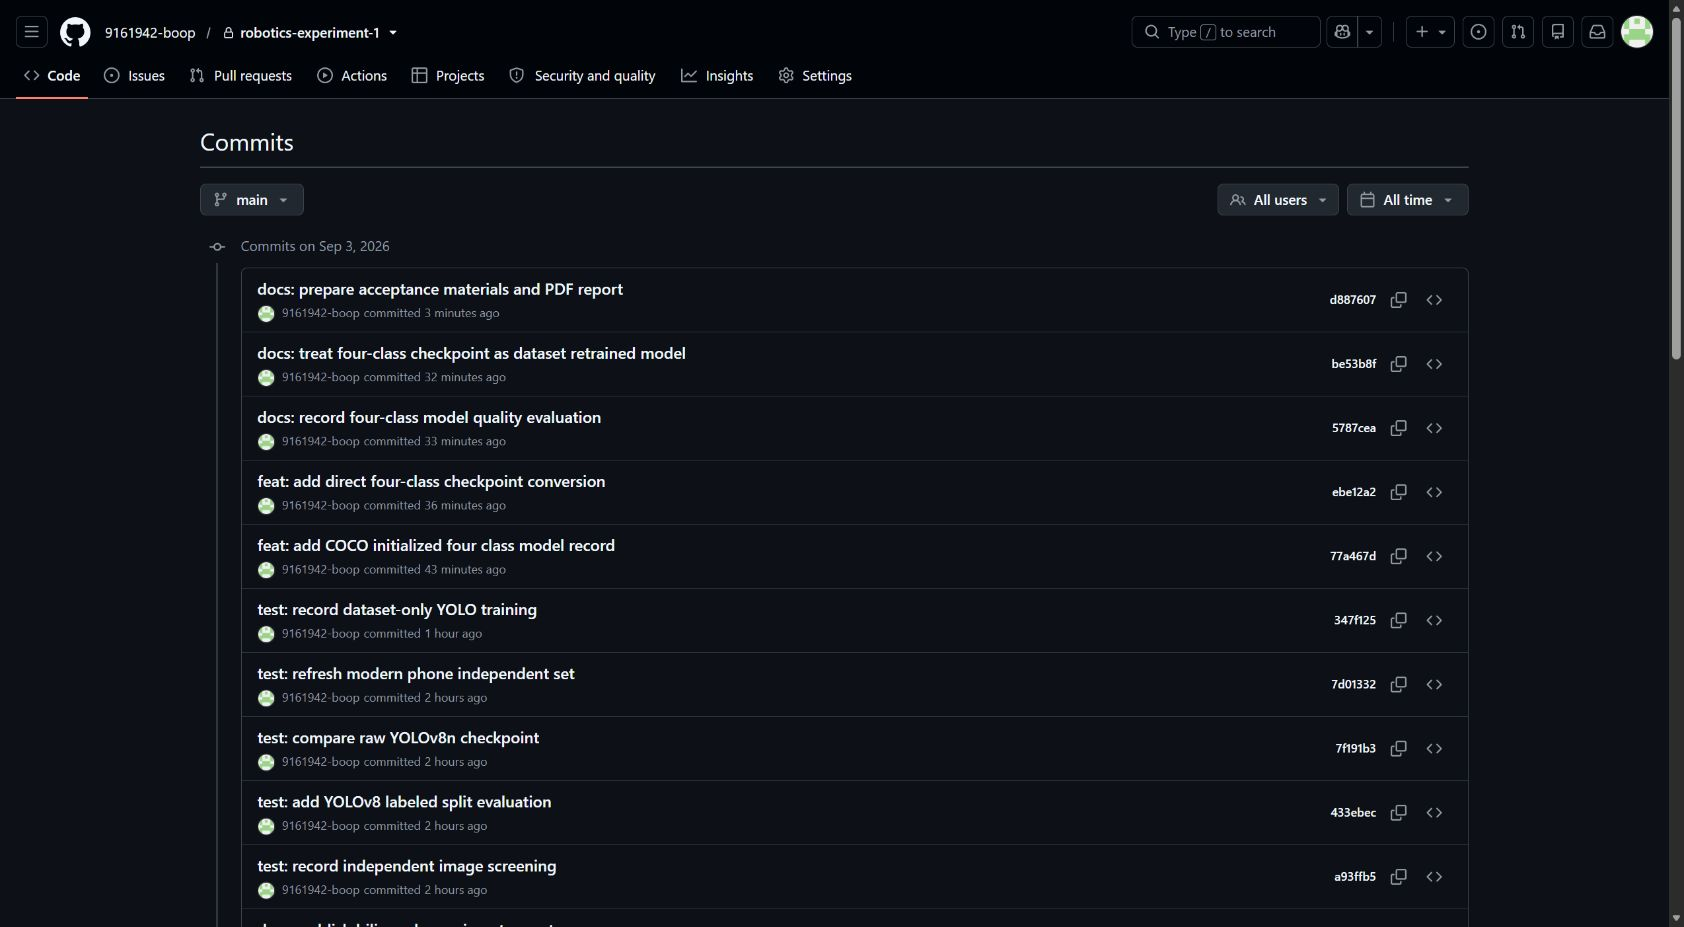
\includegraphics[width=0.98\columnwidth]{github_commit_history.png}
\tightcaption{GitHub main 分支提交记录截图（页面访问时间：2026-09-03）}
\end{figure}

\FloatBarrier
\section{提交材料与验收结论}
提交材料包括：数据集 \code{dataset/images/}、\code{dataset/yolo/}；四类模型 \code{weights/best.pt}；程序 \code{src/}、\code{scripts/}；Jetson 视频 \code{results/videos/jetson\_demo.mp4}；运行说明 \code{README.md}、\code{docs/ros2\_quickstart.md}；结果、错误案例和报告源文件。所有材料按目录整理，并通过 GitHub 分阶段 commit 留存。

\begin{table}[H]
\centering
\scriptsize
\caption{验收要求与材料证据对照}
\begin{tabularx}{\columnwidth}{>{\bfseries}p{0.27\columnwidth} X p{0.13\columnwidth}}
\toprule
验收要求 & 对应证据 & 状态\\
\midrule
同时识别不少于 2 类 & 四类模型（mouse、laptop、cup、phone）及 80 张独立照片测试记录 & 达成\\
20 个物体正确率不低于 80\% & 独立测试汇总：72/80，准确率 90\%，并附类别统计图 & 达成\\
Jetson 实时速度不低于 5 FPS & \path{results/videos/jetson_demo.mp4} 中叠加显示约 15 FPS & 达成\\
保存结果与典型错误案例 & \path{results/independent_test_80/}、\path{results/evaluation_final/} 及错误样例目录 & 达成\\
ROS2 发布识别结果 & 节点发布 \code{/detections}，启动与 \code{ros2 topic echo} 命令写入运行说明 & 已实现\\
\bottomrule
\end{tabularx}
\end{table}

\FloatBarrier
\section*{结论}
本实验完成了从数据采集、标注、YOLOv8 训练到 Jetson 实时检测和 ROS2 发布的完整链路。四类独立实物照片准确率为 90\%，Jetson 视频显示约 15 FPS，达到本实验的主要验收指标。论文式报告、源文件、数据、模型、程序、视频、运行说明和错误案例均已整理并上传 GitHub。

\flushend
\end{document}
